% !TEX root = ../main.tex

\chapter{Computing}
\label{ch:computing}

\emph{Part of this research has been described in a journal article in Digital Creativity in 2013, and I presented a paper at the Creativity and Cognition conference 2013 in Sydney.}

\grule

TEST:\\
Here’s my \gls{hyper} term. \gls{holo} \gls{hyper}\\
First use: \gls{ir}. Second use: \gls{ir}.\\
First use: \gls{nlp}. Second use: \gls{nlp}.


\section{Information Retrieval}

\begin{quote}
  "Information retrieval deals with the representation, storage, organisation of, and access to information items such as documents, Web pages, online catalogs, structured and semi-structured records, multimedia objects. The representation and organisation of the information items should be such as to provide the users with easy access to information of their interest." \citep{Baeza-Yates2011}
\end{quote}

\todo{exploratory search section}

In simple terms, a typical search process can be described as follows. A user is looking for some information so she or he types a search term or a question into the text box of a search engine. The system analyses this query and retrieves any matches from the index, which is kept up to date by a web crawler. A ranking algorithm then decides in what order to return the matching results and displays them for the user. In reality of course this process involves many more steps and level of detail, but it provides a sufficient enough overview.

From the users' point of view the search process can be broken down into four activities \citep{Sutcliffe1998} reminiscent of classic problem solving techniques \citep{Polya1957}:

\begin{description}
  \item [Problem identification]: information need (IN),
  \item [Need articulation]: IN in natural language terms,
  \item [Query formulation]: translate IN into query terms, and
  \item [Results evaluation]: compare against IN.
\end{description}

Searching can be thought of in two ways, information lookup (searching) and exploratory search (browsing) \citep{DeVries1993,Marchionini2006}. A situation where an information need cannot easily be articulated or in fact is not existent (the user is not looking for anything specific) can be considered a typical case of exploratory search and describes the kind of search that is most suited to our proposed tool.

Most big search engines like Google, Baidu or Bing focus on usefulness and relevance of their results.\citep{Google2012, Baidu2012, Microsoft2012a} Google uses over 200 signals \citep{Google2012} that influence the ranking of web pages including their original PageRank algorithm \citep{Brin1998, Brin1998b}. We can only speculate whether these signals also take into account some creative factors due to their secrecy. Other search engines like YossarianLives (currently in alpha release) \footnote{\url{http://www.yossarianlives.com/}} concentrate on purely abstract concepts like metaphors for their search algorithms.

Any information retrieval process is constrained by factors like subject, context, time, cost, system and user knowledge \citep{Marchionini1988}. Such constraints should be taken into consideration in the development of any search tool. A web crawler needs resources to crawl around the Web, language barriers may exist, the body of knowledge might not be suitable for all queries, the system might not be able to cater for all types of queries (e.g. multi-word queries), or the user might not be able to understand the user interface, and many more. It is therefore imperative to eliminate certain constraining factors (for example by choosing a specific target audience or filtering the amount of information gathered by a crawler from web pages).

Information retrieval does not only refer to the retrieval of online information from the Internet but generally also for any offline databases for example. In this survey I will focus on IR for the World Wide Web and whenever I'm speaking of an IR system I will generally refer to a web search engine system unless stated otherwise. The architecture of a search engine is made up of different components so to speak. A crawler, an indexer and a ranking system and the user interface.

\begin{figure}[htb]
  \centering
  \begin{tikzpicture}
  [every node/.style={node distance=2cm},
  box/.style={rectangle, draw, fill=black!10, inner sep=5pt, text width=2cm, text badly centered, minimum height=1cm}]
  % Coordinate Grid for testing
  % \draw[gray,very thin] (0,0) grid (6,6);
  % \foreach \x in {0,1,2,3,4,5,6}
  % \draw (\x cm,1pt) -- (\x cm,-1pt) node[anchor=north] {$\x$};
  % \foreach \y in {0,1,2,3,4,5,6}
  % \draw (1pt,\y cm) -- (-1pt,\y cm) node[anchor=east] {$\y$};
  \node [box] (web) {Web};
  \node [box, below of=web] (crawl) {Crawler};
  \node [box, below of=crawl] (index) {Index};
  \node [box, right=1cm of index] (rank) {Ranking};
  \node [box, above of=rank] (query) {Query};
  \node [box, above of=query] (user) {User};
  \path[->,thick]
  (3.375,1) edge (user.north)
  (web) edge (crawl)
  (crawl) edge (index)
  (index) edge (rank)
  (query) edge (index)
  (user) edge (query);
  \draw [->] (rank.east) -| (5,0) -- (user.east);
  \end{tikzpicture}
\caption[Search Engine Architecture]{Very abstract search engine architecture}
\label{fig:SEA}
\end{figure}

In simple terms, a typical IR process goes as follows. A user is looking for some information so he types a search term or a question into the text box of a search engine. The system then analyses that query and retrieves any matches from the index, which is always kept up to date by a web crawler in the background of the search engine. A ranking algorithm then decides in what order to return the matching results and displays them for the user. In reality this involves many more steps and levels of detail but in principle that is all needed to understand how IR systems work.


\subsection{IR Systems}

IR models describe ranking algorithms formally. There are different models for different needs, for example a multimedia IR system is going to be different than a text based IR system. Even within one such category there could more than one model. Take text based search systems for example. Text can be unstructured or semi-structured. Web pages are typically semi-structured. They contain a title, different sections or paragraphs and so on. An unstructured page would have no such differentiations but only contain simple text.  Classic example models are set theoretic, algebraic and probabilistic. The PageRank algorithm by Google is a link-based retrieval model.

The notation for IR models is as follows (quoted from \citep[p.58]{Baeza-Yates2011}):

An IR model is a quadruple $[D,Q,F,R(q_{i}, d_{j})]$ where:\\
\itab{$D$} \tab{the set of documents,}\\
\itab{$Q$} \tab{the set of queries,}\\
\itab{$F$} \tab{the framework (e.g. sets, Boolean relations, vectors, linear algebra\ldots),}\\
\itab{$R(q_{i}, d_{j})$}
\tab{the ranking function, where $q_{i} \in Q$ and $d_{j} \in D$,}\\
\itab{$t$} \tab{the number of index terms in a document collection,}\\
\itab{$V =\{k_{1},\ldots, k_{t}\}$}
\tab{is the set of all distinct index terms in a document collection (vocabulary).}

The term conjunctive component describes which terms occur ina  document and which ones do not. E.g. for $V =\{k_{1},\ldots, k_{t}\}$, if $[ k_{1},k_{2},k_{3}]$ occur in $d_{j}$ then it could be $(1,1,1)$ which means all terms occur, or $(1,0,0)$ which means only term $k_{1}$ appears in $d_{j}$.

\itab{$c(d)$} \tab{is the term conjunctive component for document $d$}\\
\itab{$c(q)$} \tab{is the term conjunctive component for query $q$}

The \textbf{term-document matrix} can be written as follows, where $f_{i,j}$ is the frequency of term $k_{i}$ in document $d_{j}$.

\begin{equation}
  \bbordermatrix{~ & d_1 & d_2 \cr
                k_1 & f_{1,1} & f_{1,2} \cr
                k_2 & f_{2,1} & f_{2,2} \cr
                k_3 & f_{3,1} & f_{3,2} \cr}
\label{eq:tdm}
\end{equation}
\myequations{tdm}

This is how an index could look like (all possible words that occur within a collection of documents), but usually an inverted index is prepared for further calculations. This inverted index is basically a list of words (the so called dictionary or vocabulary) with each word pointing to a list (the so called postings list) that indicates the documents in which the word occurs. The inverted index can include other values such as the document frequency (the number of documents that contain the term).

The dictionary is usually processed to eliminate punctuation and stop words (e.g. a, and, be, by, for, the, on, etc.) that would be useless in everyday text search engines. Techniques that are useful for this are the following \citep[Ch.2]{Manning2009}.

\begin{description}
  \item [Tokenisation] \hfill \\
  discarding white spaces and punctuation and making every term a token
  \item [Normalisation] \hfill \\
  making sets of words with same meanings, e.g. car and automobile
  \item [Case-folding] \hfill \\
  converting everything to lower case
  \item [Stemming] \hfill \\
  removing word endings, e.g. connection, connecting, connected $\to$ connect
  \item [Lemmatization] \hfill \\
  returning dictionary form of a word, e.g. went $\to$ go
\end{description}

For specific domains it even makes sense to build a "controlled vocabulary" which can be seen as a domain specific taxonomy and are very useful for query expansion.

\subsubsection{Architecture}

\subsubsection{Index}

\subsubsection{Search Algorithms}

\subsubsection{Ranking}

Ranking signals contribute to the improvement of the ranking process. These can be content signals or structural signals. Content signals are referring to anything that is concerned with the text and content of a page. This could be simple word counts or the format of text such as headings and font weights. The structural signals are more concerned about the linked structure of pages. They look at incoming and outgoing links on pages. There are also Web usage signals that can contribute to ranking algorithms such as the clickstream.  This also includes things like the Facebook "like" button or the Google+ "+1" button which could be seen as direct user relevance feedback as well.

Ranking algorithms are the essence of any web search engine and as such guarded with much secrecy. They decide which pages are listed highest in search results and if their ranking criteria were known publically, the potential for abuse (such as Google bombing \footnote{\url{http://www.searchenginepeople.com/blog/incredible-google-bombs.html}} for instance) would be much higher and search results would be less trustworthy. Despite the secrecy there are some algorithms like Google's PageRank algorithm that have been described and published in academic papers. Here is a survey of the most notable algorithms.

PageRank was developed in 1998 by Larry Page and Sergey Brin as part of their Google search engine and announced in their often cited paper \citep{Brin1998b} and they further describe the algorithm here \citep{Brin1998}. PageRank is a link analysis algorithm, meaning it looks at the incoming and outgoing links on pages. It assigns a numerical weight to each document, where each link counts as a vote of support in a sense. PageRank is executed at indexing time, so the ranks are stored with each page directly in the index. The following formula for calculating a PageRank PR is taken from \citep[p.472]{Baeza-Yates2011}.

\begin{figure}[htb] % (here, top, bottom, page)
  \centering
  \includegraphics[width=\linewidth]{pagerank}
\caption[PageRank algorithm]{PageRank algorithm from Wikipedia}
\label{fig:pagerank}
\end{figure}

\begin{equation}
  PR(a) =
  \frac{q}{T} + (1 - q)
  \sum_{i=1}^{n} \frac{PR(p_i)}{L(p_i)}
  \label{eq:PR}
\end{equation}
\myequations{PR}

Where,\\
\itab{$L(p)$} \tab{is the number of outgoing links of page $p$}\\
\itab{$a$} \tab{is the page we want to rank and is pointed to by pages $p_1$ to $p_n$}\\
\itab{$T$} \tab{is the total number of pages on the Web graph}\\
\itab{$q$} \tab{is the is a parameter to be set by the system (typically 0.15)}\\
\itab{} \tab{needed to deal with dead ends in the graph}

The HITS algorithm also works on the links between pages. It was first described by Kleinberg \citep[p.472]{Kleinberg1999, Kleinberg} in 1999. HITS stands for Hyperlink Induced Topic Search and its basic features are the use of so called hubs and authority pages. It is executed at query time. Pages that have many incoming links are called authorities and page with many outgoing links are called hubs. Again, the following formula is taken from \citep[p.471]{Baeza-Yates2011}. S is the set of pages.

\begin{equation}
  \begin{split}
  H(p) &= \sum_{u\in S \mid p\to u}A(u)\\
  A(p) &= \sum_{v\in S \mid v\to p}H(v)
  \end{split}
  \label{eq:HITS}
\end{equation}
\myequations{HITS}

Hilltop is a similar algorithm with the difference that it operates on a specific set of expert pages as a starting point. It was defined by Bharat and Mihaila in 2000 in \citep{Bharat2000}. The expert pages they refer to should have many outgoing links to non-affiliated pages on a specific topic. This set of expert pages needs to be pre-processed at the indexing stage. The authority pages they define must be linked to by one of their expert pages. The main difference to the HITS algorithm then is that their "hub" pages are predefined.

Another algorithm is the so called Fish search algorithm. It was first described by De Bra in 1994 \citep{Debra1994, Debra1994a, Debra}. The basic concept here is that the search starts with the search query and a seed URL as a starting point. A list of pages is then built dynamically in order of relevance following from link to link. Each node in this directed graph is given a priority depending on whether it is judged to be relevant or not. URLs with higher priority are inserted at the front of the list while others are inserted at the back. Special here is that the "ranking" is done dynamically at query time.

There are various algorithms that follow this approach. For example the shark search algorithm \citep{Hersovici1998}. It improves the process of judging whether or not a given link is relevant or not. It uses a simple vector model with a fuzzy sort of relevance feedback. Another example is the improved fish search algorithm in \citep{Luo2005} where the authors have simply added an extra parameter to allow more control over the search range and time. The Fish School Search algorithm is another approach based on the same fish inspiration \citep{BastosFilho2008}. It uses principles from genetic algorithms and particle swarm optimization. Another genetic approach is Webnaut \citep{Nick2001}.

Other variations include the incorporation of user behaviour \citep{Agichtein2006}, social annotations \citep{Bao2007}, trust \citep{Garcia-Molina2004}, query modifications \citep{Glover2001}, topic sensitive PageRank [59](p430) \citep{Haveliwala2003}, folksonomies \citep{Hotho}, SimRank \citep{Jeh}, neural-networks \citep{Shu1999}, and semantic web \citep{Widyantoro2001,Du2007,Ding,Kamps,Taye2009}.


\subsection{Evaluation}

\subsubsection{Measuring Search Quality}

Evaluating search results is not easy. The most widely used metric to measure the quality of results is that of precision and recall.

Precision is defined as the fraction of retrieved documents that are relevant.

\begin{equation}
  Precision = \frac{relevant documents retrieved}{retrieved documents}
  \label{eq:precision}
\end{equation}
\myequations{precision}

Recall is defined as the fraction of relevant documents that are retrieved.

\begin{equation}
  Recall = \frac{relevant documents retrieved}{relevant documents}
  \label{eq:recall}
\end{equation}
\myequations{recall}

Note the slight difference between the two. Precision tells us how many of all retrieved results were actually relevant (of course this should preferable be very high) and recall simply indicates how many of all possible relevant documents we managed to retrieve. This can be easily visualised as follows.

% Definition of circles
\def\leftcircle{(0,0) circle (1.5cm)}
\def\rightcircle{(0:2cm) circle (1.5cm)}
\colorlet{circle edge}{black!50}
\colorlet{circle area}{black!20}
\tikzset{filled/.style={fill=circle area, draw=circle edge, thick},
    outline/.style={draw=circle edge, thick}}

\begin{figure}[htb]
  \centering
  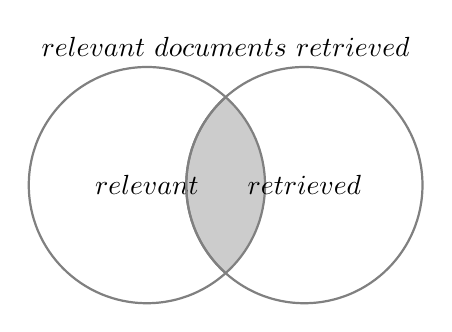
\begin{tikzpicture}
  \begin{scope}
  \clip \leftcircle;
  \fill[filled] \rightcircle;
  \end{scope}
  \draw[outline] \leftcircle node {$relevant$};
  \draw[outline] \rightcircle node {$retrieved$};
  \node[anchor=south] at (current bounding box.north) {$relevant \ documents \ retrieved$};
  \end{tikzpicture}
\caption[Precision and Recall]{Precision and Recall}
\label{fig:PR}
\end{figure}

Precision is typically more important than recall in web search while it is the other way around in a database search system maybe. The mean average precision value (MAP) can be calculated following this formula (taken from \citep[p.141]{Baeza-Yates2011}:

\begin{equation}
  MAP_i = \frac{1}{|R_i|} \sum_{k=1}^{|R_i|} P(R_i[k])
  \label{eq:MAP}
\end{equation}
\myequations{MAP}

Where $R_i$ is the set of relevant documents for query $q_i$.

But for many web searches is it not necessary to calculate the average of all results, since users don't inspect results after the first page very often and it is therefore desirable to have the highest level of precision in the first 5 to 30 results maybe. For this purpose it is common to measure the average precision of web search engines after only a few documents have been seen. This is called "Precision at n" or "P@n" \citep[p.140]{Baeza-Yates2011}. So for example this could be P@5 or P@10 or P@20. For example, to compare two ranking algorithms, we would calculate P@10 for each of them over an average of 100 queries maybe and compare the results and therefore the performance of the algorithm.

The Text REtrieval Conference (TREC) is a conference that provides large test sets of data to participants and lets them compare results. They have specific test sets for web search comprised of crawls of .gov web pages for example, but unfortunately they have to paid for to get a copy. \footnote{\url{http://ir.dcs.gla.ac.uk/test_collections/}}

There are certain other factors that can be or need be evaluated when looking at the complete search system. For example the time it takes to crawl for data, the time it takes to index data, the amount of storage needed for data and then also how fast the query response is and how many queries the system can handle in a given time period.


\subsubsection{Measuring Creative Search Quality}

In this paper \citep{Sawle2011} we have discussed an initial approach to measure the creativity of search results. Based on a definition of creativity by Boden, we attempt to define creativity in a way which could be applied to search results and provide a simple metric to measure it.


\subsubsection{Query Expansion and Relevance Feedback}

Relevance feedback is an idea of improving the search results by explicit or implicit methods. Explicit feedback asks users to rate results according to their relevance or collects that kind of information through analysis of mouse clicks, eye tracking etc. Implicit feedback occurs when external sources are consulted such as thesauri or by analysis the top results provided by the search engine. There are two ways of using this feedback. It can be displayed as a list of suggested search terms to the user and the user decided whether or not to take the advice, or the query is modified internally without the user's knowledge. This is then called automatic query expansion.


\subsection{The Boolean Model}

The similarity of document $d_j$ to query $q$ is defined as follows (quoted from \citep[p.65]{Baeza-Yates2011})

\begin{equation}
  sim(d_j,q) =
  \begin{cases}
  1 & \text{if} \ \exists \ c(q) \ | \ c(q) = c(d_j)\\
  0 & \text{otherwise}
  \end{cases}
  \label{eq:sim}
\end{equation}
\myequations{sim}

Sometimes things are not quite black and white though and we need to weigh the importance of words somehow. The easiest way to do that is by looking at the frequency in which a word occurs.


\subsection{The Vector Model}

The vector model allows a more flexible scoring since it basically computes the various degrees of similarity between documents (taken from \citep[p.78]{Baeza-Yates2011}).

\begin{equation}
  \begin{split}
  \vec{d_j} &= (w_{1,j}, w_{2,j}, \ldots, w_{t,j})\\
  \vec{q} &= (w_{1,q}, w_{2,q}, \ldots, w_{t,q})
  \end{split}
  \label{eq:vector}
\end{equation}
\myequations{vector}

\begin{figure}[htb] % (here, top, bottom, page)
  \centering
  \begin{tikzpicture}
  \draw
  (3,0) coordinate (a) node[right] {$q$}
  -- (0,0) coordinate (b) node[left] {}
  -- (2,2) coordinate (c) node[above right] {$d_j$}
  pic["$\theta$", draw=black, angle eccentricity=1.2, angle radius=1cm]
  {angle=a--b--c};
  \end{tikzpicture}
\caption[Vector Model]{The Vector Model}
\label{fig:VM}
\end{figure}

Where $t$ is the total number of terms in the index and $w_{i,j}$ is the TF-IDF weight for each component of the vector. The similarity between the document and the query vector is the cosine of $\theta$.

\begin{equation}
  \begin{split}
  sim(d_j,q) &= \frac{\vec{d_j} \ \cdot \ \vec{q}}{|\vec{d_j}| \times |\vec{q}|}\\
  &= \frac{\sum_{i=1}^{t}w_{i,j} \times w_{i,q}}
  {\sqrt{\sum_{i=1}^{t}w_{i,j}^{2}} \times \sqrt{\sum_{i=1}^{t}w_{i,q}^{2}}}
  \end{split}
  \label{eq:sim2}
\end{equation}
\myequations{sim2}

Here is an example algorithm for computing this score taken from \citep[p.125]{Manning2009}.

\begin{figure}[htb]
  \begin{lstlisting}
  CosineScore(q)
    float Scores[N] = 0
    for each d
    do Initialise Length[d] to the length of document d
    for each query term t
    do calculate wt,q and fetch postings list for t
      for each pair(d, tft,d) in postings list
      do add wft,d to Scores[d]
    Read the array Length[d]
    for each d
    	do Divide Scores[d] by Length[d]
    	return Top K components of Scores[]
  \end{lstlisting}
\caption[Pseudo-code for computing vector scores]{Pseudo-code for computing vector scores}
\label{fig:VectorScores}
\end{figure}

Where,\\
\itab{$q$} \tab{is the query}\\
\itab{$N$} \tab{is the total number of documents}\\
\itab{$d$} \tab{is a document}\\
\itab{$t$} \tab{is a query term}\\
\itab{$wt_q$} \tab{is the weight of the term in the query}\\
\itab{$tft_d$} \tab{is the term frequency of $t$ in $d$}\\
\itab{$wft_d$} \tab{is the $tf-idf$ weight of t in $d$}\\
\itab{$K$} \tab{is the number of results we want}\\
\itab{$postings list$} \tab{is the list of all ($d$, $tft_d$) for a given $t$.}

There are several other common IR models that I won't discuss in detail here. These include the probabilistic, set-based, extended Boolean and fuzzy set \citep{Miyamoto2010, Miyamoto1988, Srinivasan2001, Widyantoro2001, Miyamoto1986} models or latent semantic indexing \citep{Deerwester1990}, neural network models and others \citep{Macdonald2009, Schuetze1998, Schuetze}.


\subsection*{Total Term Frequency}

\begin{equation}
  F_i = \sum_{j=1}^{N}f_{i,j}
  \label{eq:Fi}
\end{equation}
\myequations{Fi}

Where $F_i$ is the total frequency of term $k_i$ in the collection and $f_{i,j}$ is the frequency of occurance of term $k_i$ in document $d_j$ and $N$ is the total number of documents.


\subsubsection*{Term Frequency TF}

normalised using log function

\begin{equation}
  tf_{i,j}=
  \begin{cases}
  1+\log f_{i,j} & \text{if} \ f_{i,j} > 0\\
  0 & \text{otherwise}
  \end{cases}
  \label{eq:tfij}
\end{equation}
\myequations{tfij}


\subsubsection*{Inverse Document Frequency IDF}

\begin{equation}
  idf_j = \log \frac{N}{df_i}
  \label{eq:idfj}
\end{equation}
\myequations{idfj}

Where the document frequency $df_i$ is the number of documents in a collection that contain a term $k_i$ and $idf_i$ is the IDF of term $k_i$. The more often a term occurs in different documents the lower the IDF.


\subsubsection*{TF-IDF Weighting}

\begin{equation}
  w_{i,j} =
  \begin{cases}
  (1+\log f_{i,j})\times \log\frac{N}{df_i} & \text{if} \ f_{i,j} > 0 \\
  0 & \text{otherwise}
  \end{cases}
  \label{eq:wij}
\end{equation}
\myequations{wij}

Where $w_{i,j}$ is the weight associated with $(k_i,d_j)$. In simpler notation this is:

\begin{equation}
  w_{i,j} = tf_{i,j}\times idf_j
  \label{eq:wij2}
\end{equation}
\myequations{wij2}

This means that rare terms have a higher weight and more so if they occur a lot in one document.


\subsubsection*{Challenges of Web Search}

Other issues that arise when trying to search the World Wide Web are as follows (\citep[p.449]{Baeza-Yates2011}).

\begin{itemize}
  \item Data is distributed. Data is located on different computers all over the world and network traffic is not always reliable.
  \item Data is volatile. Data is deleted, changed or lost all the time so data is often out-of-date and links broken.
  \item The amount of data is massive and grows rapidly. Scaling of the search engine is an issue here.
  \item Data is often unstructured. There is no consistency of data structures.
  \item Data is of poor quality. There is no editor or censor on the Web. A lot of data is redundant too.
  \item Data is not heterogeneous. Different data types (text, images, sound, video) and different languages exist.
\end{itemize}

Since a single query for a popular word can results in  millions of retrieved documents from the index, search engine usually adopt a lazy strategy, meaning that they only actually retrieve the first few pages of results and only compute the rest when needed \citep[p.459]{Baeza-Yates2011}. To handle the vast amounts of space needed to store the index, big search engines use a massive parallel and cluster-based architecture \citep[p.459]{Baeza-Yates2011}. Google for example uses over 15,000 commodity-class PCs that are distributed over several data centres around the world \citep{Dean2003}.


\subsubsection*{Summary}

IR refers to the retrieval of information from a collection. In terms of the Internet it is often called Web search. A Web search engine is divided into different components, being the crawler to build an index of the collection and a ranking algorithm which stands between the index and the user.

Different retrieval models exist including the Boolean and the Vector model. Other methods exist to make search results more accurate, including relevance feedback and query expansion.

Search quality is generally measured using the metrics of precision and recall but for Web search precision is more important and usually a metric called "precision at n" is used for measurements.

Challenges are the size of the World Wide Web and ambiguous, unstructured nature of Web pages among others.

Ranking can be done at different stages of the search process. Depending on how the index is formatted and what information can be pre-computed at that stage, the ranking algorithm evaluates every page for relevance and returns them in order. There exist lots of different approaches on ranking, including PageRank and HITS (both analyse the link structure of the WWW), or more dynamic models like Fish search or genetic approaches.


\section{Natural Language Processing}

\begin{comment}
  Damerau-Levensthein for clinamen!
\end{comment}

Bird, S., Klein, E. and Loper, E., 2009. NLP with Python 1st ed., Sebasopol, CA: O'Reilly Media.\citep{Bird2009}

Manning, C., Raghavan, P. and Schuetze, H., 2008. Introduction to Information Retrieval 1st ed., Cambridge: Cambridge University Press.\citep{Manning2009}

Taken from [1]:\citep{Jurafsky2009}\\
Also known as:\\
\begin{itemize}
  \item Speech and language processing
  \item Human language technology
  \item Natural language processing (NLP)
  \item Computational linguistics
  \item Speech recognition and synthesis
\end{itemize}

Goals of NLP are to get computers to perform useful tasks involving human language like:
\begin{itemize}
  \item Enabling human-machine communication
  \item Improving human-human communication
  \item Text and speech processing
\end{itemize}

e.g. machine translation, automatic speech recognition, natural language understanding, word sense disambiguation, spelling correction, grammar checking…


\subsection{Damerau-Levensthein}


\subsection*{Regular Expressions}

Used to specify text strings in text.

RE search requires a pattern that we want to search for and a corpus of texts to search through.

Errors can be false positives (FP) and false negatives (FN).

\begin{itemize}
  \item Increasing accuracy (minimizing FP)
  \item Increasing coverage (minimizing FN)
\end{itemize}

RE's can be expressed as Finite-State Automata (FSA).


\subsection*{Language Models (LM)}

Probabilities are based on counting things. Counting things in natural language is based on a corpus (pl corpora), a computer readable collection of text or speech.

Cats versus cat?

Same lemma but different wordforms.

\begin{itemize}
  \item A lemma is a set of lexical forms that have the same stem. (e.g. go)
  \item A wordform is the full inflected or derived form of the word. (e.g. goes)
  \item A word type is a distinct word in a corpus (repetitions are not counted but case sensitive).
  \item A word token is any word (repetitions are counted repeatedly)
\end{itemize}

The process of converting all words in a text to their lemma (e.g. goes $\to$ go) is called lemmatisation and the process of separating out all words in a text is called tokenisation or word segmentation.


\subsection*{$N$-Grams}

We can do word prediction with probabilistic models called $N$-Grams. They predict the probability of the next word from the previous $N-1$ words.

We want to compute the probability for $P(w|h)$ where $w$ is a word and $h$ is a history (the previous words). How many times occurred h followed by $w$ divided by how many times occurred $h$?

\begin{equation}
  P(w \mid h) = \frac{count(hw)}{count(h)}
  \label{eq:Probwh}
\end{equation}
\myequations{Probwh}

Using the \textbf{chain rule of probability}:

\begin{equation}
  \begin{split}
  P(w_1^n) &= P(w_1)P(w_2 \mid w_1)P(w_3 \mid w_1^2 ) \ldots P(w_n \mid w_1^{n-1})\\
  &= \prod_{k=1}^{n}P(w_k \mid w_1^{k-1})
  \end{split}
  \label{eq:Probw1n}
\end{equation}
\myequations{Probw1n}

Using the \textbf{Markov assumption} that probability of a word depends only on the previous word (or $n$ words).

\begin{equation}
  P(w_1^n) = \prod_{k=1}^{n}P(w_k \mid w_{k-1})
  \label{eq:Probw1n2}
\end{equation}
\myequations{Probw1n2}

Using the \textbf{maximum likelihood estimation (MLE)} for $N$-Grams we can normalise counts to be between 0 and 1. $C$ stands for count.


\subsection*{Maximum likelihood estimation (MLE)}

\begin{equation}
  P(w_n \mid w_{n-N+1}^{n-1}) = \frac{C(w_{n-N+1}^{n-1} w_n)}{C(w_{n-N+1}^{n-1})}
  \label{eq:Probwn}
\end{equation}
\myequations{Probwn}

Usually instead of calculating the counts based on products we calculate them based on sums of logs.

So instead of  $p_1 \times p_2 \times p_3 \times p_4 = \log p_1 + \log p_2 + \log p_3 + \log p_4$

Google offers its $N$-Gram data for free on:

\begin{itemize}
  \item \url{http://bit.ly/1baDXAW} % http://googleresearch.blogspot.co.uk/2006/08/all-our-n-gram-are-belong-to-you.html
  \item \url{http://books.google.com/ngrams/}
  \item	\url{http://www.speech.sri.com/projects/srilm/}
  \item	\url{http://bit.ly/1G3ZJmX} % http://www.ldc.upenn.edu/Catalog/CatalogEntry.jsp?catalogId=LDC2006T13
\end{itemize}


\subsection*{Evaluating N-Grams}

Extrinsic and intrinsic evaluation.

\begin{description}
  \item [Extrinsic]: evaluate performance of a language model by embedding it into an independent application.
  \item [Intrinsic]: evaluate independent on any application, e.g. perplexity.
\end{description}


\subsection*{Perplexity}

\begin{equation}
  PP(W) = \sqrt[N]{\prod_{i=1}^{N}\frac{1}{P(w_i \mid w_{i-1})}}
  \label{eq:ppw}
\end{equation}
\myequations{ppw}


\subsection*{Smoothing}


\subsection*{Add-One : Laplace smoothing  for bigrams}

\begin{equation}
  P_{Add-1}(w_i \mid w_{i-1}) = \frac{c(w_{i-1}, w_i) + 1}{c(w_{i-1}) + V}
  \label{eq:padd1}
\end{equation}
\myequations{padd1}


\subsection*{Adjusted count}

\begin{equation}
  c_i^* = (c_i+1)\frac{N}{N+V}
  \label{eq:ci}
\end{equation}
\myequations{ci}

Add-1 smoothing is ok for text categorisation but not so much for language modelling.

Most commonly used is Kneser-Ney extended interpolated.

For very large N-grams like the Web “Stupid Backoff” is used.


\subsection*{Good Turing Discounting}

$N_c$ is the frequency of frequency $c$.

\begin{equation}
  c^* = (c+1)\frac{N_{c+1}}{N_c}
  \label{eq:cstar}
\end{equation}
\myequations{cstar}


\subsection*{Naive Bayes}

[3] page 234…

\begin{quote}
  (Wikipedia): "A naive Bayes classifier is a simple probabilistic classifier based on applying Bayes' theorem with strong (naive) independence assumptions. A more descriptive term for the underlying probability model would be 'independent feature model'."
\end{quote}


\subsection*{Maximum Entropy Models (MaxEnt)}

Page 227 .. in [1]

MaxEnt models are also widely known as \textbf{multinomial logistic regression}. They are used for sequence classification, e.g. part-of-speech tagging. They belong to a family of classifiers known as \textbf{exponential or log-linear classifiers}.

The task of classification is to take a single observation, extract some useful features describing the observation, and then, based on these features, to classify the observation into one of a set of discrete classes. A probabilistic classifier also gives the probability of the observation being in that class; it gives a probability distribution over all classes.

MaxEnt works by extracting some set of features from the input, combining them linearly (meaning that each feature is multiplied by a weight and then added up), and then using this sum as an exponent.
Formula below shows how to calculate the probability of class $c$ given an observed datum (a given data point) $d$ and $\lambda$ is a weight that is assigned to feature $f$. Taking the exponent makes the result always positive. Dividing by the Sum of that for all classes makes it a probability.

\begin{equation}
  P(c \mid d, \lambda) = \frac{\exp\sum_i\lambda_i f_i (c,d)}{\sum_{c\prime}\exp\sum_{i}\lambda_i f_i (c\prime,d))}
  \label{eq:pcdlambda}
\end{equation}
\myequations{pcdlambda}

To get the single best class with the highest probability we need to compute the following.

\begin{equation}
  \hat{c} = \underset{c\in C}{\text{argmax}} \ P(c \mid d,\lambda)
  \label{eq:hatc}
\end{equation}
\myequations{hatc}

\begin{table}[htb]
  \centering
  \begin{tabu}{lll}
  \toprule
  PERSON    & LOCATION   & DRUG      \\ \midrule
  In Québec & In Québec  & In Québec \\
  0         & 1.8 + -0.6 & 0.3       \\
  \bottomrule
  \end{tabu}
\caption[MaxEnt Example table]{MaxEnt Example table}
\label{tab:maxent}
\end{table}

Features:

$f1(c,d) \equiv [ \ c = \text{LOCATION} \ \wedge \ w-1 = \text{``in"} \wedge \ \text{isCapitalized}(w)]$\\
$f2(c,d) \equiv [ \ c = \text{LOCATION} \ \wedge \ \text{hasAccentedLatinChar}(w)]$\\
$f3(c,d) \equiv [ \ c = \text{DRUG} \ \wedge \ \text{ends}(w,\text{``c"})]$

$P(\text{LOCATION} \mid \text{in Québec}) = \frac{e^{1.8} e^{–0.6}}{e^{1.8} e^{–0.6} + e^{0.3} + e^0} = 0.586$\\
$P(\text{DRUG} \mid \text{in Québec}) = \frac{e^{0.3}}{e^{1.8} e^{–0.6} + e^{0.3} + e^0} = 0.238$\\
$P(\text{PERSON} \mid \text{in Québec}) = \frac{e^0}{e^{1.8} e^{–0.6} + e^{0.3} + e^0} = 0.176$

The empirical expectation is the sum of all occurrences where a feature is true for one of our observed datums.

\begin{equation}
  empirical \ E(f_i)= \sum_{(c,d) \ \in \ observed(C,D)}f_i(c,d)
  \label{eq:epirical}
\end{equation}
\myequations{epirical}


\subsection*{Evaluation}

\begin{equation}
  Precision = \frac{\text{number of correctly labeled}}{\text{total number of extracted}}
  \label{eq:preci}
\end{equation}
\myequations{preci}

\begin{equation}
  Recall = \frac{\text{number of correctly labeled}}{\text{total number of gold}}
  \label{eq:reca}
\end{equation}
\myequations{reca}

\begin{equation}
  F_1 = \frac{2PR}{P+R}
  \label{eq:f1mes}
\end{equation}
\myequations{f1mes}


\subsection*{Information Extraction}

[1] Chapter 22, p 759…

"The process of information extraction (IE), also called text analytics, turns the unstructured information embedded in texts into structured data."

IE involves named entity recognition (NER), relation detection and classification, event detection and classification and temporal analysis.


\subsection*{Named Entity Recognition}

A named entity can be anything that can be referred to by a proper name, such as person-, place- or organisation names and times and amounts.

Example (first sentence in Faustroll):

\begin{quote}
  "In this year Eighteen Hundred and Ninety-eight, the Eighth day of February, Pursuant to article 819 of the Code of Civil Procedure and at the request of M. and Mme. Bonhomme (Jacques), proprietors of a house situate at Paris, 100 bis, rue Richer, the aforementioned having address for service at my residence and further at the Town Hall of Q borough."
\end{quote}

\begin{quote}
  In this $[$year Eighteen Hundred and Ninety-eight, the Eighth day of February$]^{\text{TIME}}$, Pursuant to article $[$819$]^{\text{NUMBER}}$ of the $[$Code of Civil Procedure$]^{\text{DOCUMENT}}$ and at the request of $[$M. and Mme. Bonhomme (Jacques)$]^{\text{PERSON}}$, proprietors of a house situate at $[$Paris, 100 bis, rue Richer$]^{\text{LOCATION}}$, the aforementioned having address for service at my residence and further at the $[$Town Hall$]^{\text{FACILITY}}$ of $[$Q borough$]^{\text{LOCATION}}$.
\end{quote}

Gazetteers (lists of place or person names for example) can help with the detection of these named entities.


\subsection*{Part of Speech Tagging}

Parts of speech (POS) are lexical tags for describing the different elements of a sentence. The eight main parts-of-speech (originating from ca. 100 B.C.) are noun, verb, pronoun, preposition, adverb, conjunction, participle and article.
Wikipedia:

\begin{description}
  \item [Noun]: any abstract or concrete entity; a person (police officer, Michael), place (coastline, London), thing (necktie, television), idea (happiness), or quality (bravery)
  \item [Pronoun]: any substitute for a noun or noun phrase
  \item [Adjective]: any qualifier of a noun
  \item [Verb]: any action (walk), occurrence (happen), or state of being (be)
  \item [Adverb]: any qualifier of an adjective, verb, or other adverb
  \item [Preposition]: any establisher of relation and syntactic context
  \item [Conjunction]: any syntactic connector
  \item [Interjection]: any emotional greeting (or "exclamation")
\end{description}

Building a Large Annotated Corpus of English \citep{Marcus1993}

There exist other sets of tags, like the Penn Treebank with divides those 8 tags into a total of 45, for example $CC$ for coordinating conjunction, $CD$ for cardinal number, $NN$ for noun singular, $NNS$ for noun plural, $NNP$ for proper noun singular, $VB$ for verb base form, $VBG$ for verb gerund, etc.

The process of adding tags to the words of a text is called parts-of-speech tagging or just tagging. This usually is done together with the tokenisation of the text.

Example (first sentence in Faustroll):

\begin{quote}
  In\slash IN this\slash DT [year\slash NN Eighteen\slash CD Hundred\slash CD and\slash CC Ninety-eight\slash CD,\slash , the\slash DT Eighth\slash CD day\slash NN of\slash IN February\slash NNP]$^{\text{TIME}}$,\slash , Pursuant\slash JJ to\slash IN article\slash NN [819\slash  CD]$^{\text{NUMBER}}$ of\slash IN the\slash DT [Code\slash NN of\slash IN Civil\slash NNP Procedure\slash NNP]$^{\text{DOCUMENT}}$ and\slash CC at\slash IN the\slash DT request\slash NN of\slash IN [M.\slash NN and\slash CC Mme.\slash NN Bonhomme\slash NNP (\slash (Jacques\slash NNP)\slash )]$^{\text{PERSON}}$,\slash , proprietors\slash NNS of\slash IN a\slash DT house\slash NN situate\slash JJ at\slash IN [Paris\slash NNP,\slash , 100\slash CD bis\slash NN ,\slash , rue\slash NN Richer\slash NNP]$^{\text{LOCATION}}$,\slash , the\slash DT aforementioned\slash JJ having\slash VBG address\slash NN for\slash IN service\slash NN at\slash IN my\slash PRP residence\slash NN and\slash CC further\slash JJ at\slash IN the\slash DT [Town\slash NNP Hall\slash NNP]$^{\text{FACILITY}}$ of\slash IN [Q\slash NNP borough\slash NN]$^{\text{LOCATION}}$.\slash .
\end{quote}

\begin{equation}
  t_1^n = \underset{t_1^n}{\text{argmax}} \ P(w_1^n \mid t_1^n) P(t_1^n)
  \label{eq:tn1}
\end{equation}
\myequations{tn1}

\begin{equation}
  P(t_i \mid t_{i-1}) = \frac{C(t_{i-1},t_i)}{C(t_{i-1})}
  \label{eq:pti}
\end{equation}
\myequations{pti}

For example: the probability of getting a common noun after a determiner is:

\begin{equation}
  P(\text{NN} \mid \text{DT}) = \frac{C(\text{DT},\text{NN})}{C(\text{DT})} = \frac{56,509}{116,454} = 0.49
  \label{eq:pnndt}
\end{equation}
\myequations{pnndt}

Given that there are 116,454 occurrences of DT in the corpus and of these 56,509 occurrences where a NN follows after the DT.

\begin{equation}
  P(\text{is} \mid \text{VBZ}) = \frac{C(\text{VBZ},\text{is})}{C(\text{VBZ})} = \frac{10,073}{21,627} = 0.47
  \label{eq:pisvbz}
\end{equation}
\myequations{pisvbz}

Or the probability of a third person singular verb being 'is' is 0.47.


\subsection*{Parsing}

Parsing is the process of analysing a sentence and assigning a structure to it. Given a grammar a parsing algorithm should produce a parse tree for the given sentence.


\subsection*{Grammar}

A language is modelled using a grammar, specifically a Context-Free-Grammar or CFG. Such a grammar normally consists or rules and a lexicon. For example a rule could be NP $\to$ Det Noun, where NP stands for noun phrase, Det for determiner and Noun for a noun. The corresponding lexicon would then include facts like Det $\to$ a, Det $\to$ the, Noun $\to$ book. This grammar would let us form the noun phrases "the book" and "a book" only. The two parse trees would then look like this:

\begin{figure}[htb]
  \centering
  \begin{minipage}{.4\linewidth}
  \Tree[.NP [.Det \textit{a} ]
  [.Noun \textit{book} ]]
  \end{minipage}
  \hspace{.05\linewidth}
  \begin{minipage}{.4\linewidth}
  \Tree[.NP [.Det \textit{the} ]
  [.Noun \textit{book} ]]
  \end{minipage}
\caption[Grammers]{Grammers}
\label{Grammers}
\end{figure}

The parse tree for the previous example sentence from Faustroll is shown below, in horizontal for convenience.

\begin{alltt}
(ROOT
  (S
    (PP (IN In)
      (NP (DT this) (NN year) (NNPS Eighteen) (NNP Hundred)
        (CC and)
        (NNP Ninety-eight)))
    (, ,)
    (NP
      (NP (DT the) (JJ Eighth) (NN day))
      (PP (IN of)
        (NP (NNP February) (, ,) (NNP Pursuant)))
      (PP
        (PP (TO to)
          (NP
            (NP (NN article) (CD 819))
            (PP (IN of)
              (NP
                (NP (DT the) (NNP Code))
                (PP (IN of)
                  (NP (NNP Civil) (NNP Procedure)))))))
        (CC and)
        (PP (IN at)
          (NP
            (NP (DT the) (NN request))
            (PP (IN of)
              (NP (NNP M.)
                (CC and)
                (NNP Mme) (NNP Bonhomme))))))
      (PRN (-LRB- -LRB-)
        (NP (NNP Jacques))
        (-RRB- -RRB-))
      (, ,)
      (NP
        (NP (NNS proprietors))
        (PP (IN of)
          (NP
            (NP (DT a) (NN house) (NN situate))
            (PP (IN at)
              (NP (NNP Paris))))))
      (, ,)
      (NP (CD 100) (NN bis))
      (, ,))
    (VP (VBP rue)
      (NP
        (NP (NNP Richer))
        (, ,)
        (NP (DT the) (JJ aforementioned)
          (UCP
            (S
              (VP (VBG having)
                (NP
                  (NP (NN address))
                  (PP (IN for)
                    (NP (NN service))))
                (PP (IN at)
                  (NP (PRP$ my) (NN residence)))))
            (CC and)
            (PP
              (ADVP (RBR further))
              (IN at)
              (NP
                (NP (DT the) (NNP Town) (NNP Hall))
                (PP (IN of)
                  (NP (NNP Q))))))
          (NN borough))))
    (. .)))
\end{alltt}

This particular tree was generated using the Stanford Parser at \url{http://nlp.stanford.edu:8080/parser/index.jsp}.
Given the rather complicated nature of the words and sentence structure, some of the labels might be wrong.


\section{Linguistics / WordNet}

I looked into linguistics for the purpose of patadata. This section definitely needs some expanding. Some concepts that might be relevant include (taken from Wikipedia):

\begin{description}
  \item [Hyponym] – subcategory of something
  \item [Hypernym] – top category of some things
  \item [Meronym] – member of something (e.g. finger is meronym to hand, wheel to car)
  \item [Holonym] – e.g. tree is holonym of bark, trunk, limb… opposite of meronym
  \item [Troponym] – presence of “manner” between things (e.g. to traipse and to mince = walk a certain way)
  \item [Homonym] – same spelling but different sound and meaning = heteronym – same sound but different spelling = heterography – same meaning = synonym
  \item [Antonym] – opposite
  \item [Metonym] – figure of speech (e.g. Hollywood for American movies) not quite metaphor but similar.
\end{description}

I need to find REFERENCES for this section.

% For a project of this kind of speciality, it is hard to find directly related work. There is no real  precedent to the idea of a pataphysical search tool.
% Looking at more broadly related work shows a few worthwhile mentions as follows. They are mostly examples of creative computing in various forms, some of which have pataphysical foundations, whether they are aware of it or not, and others don't. The list could be extended endlessly, so I will only include a selection of the most interesting ones. I have also included some examples of other kinds of projects that have pataphysical elements in them but are not related to computers or searching. Finally, I have added a few examples of current web search engines and ranking algorithms, though they probably cannot be considered creative or pataphysical.


\section*{SpecLab}

The projects Johanna Drucker describes in her book SpecLab \citep{Drucker2009}  could certainly be considered related work. Not only in their theoretical foundations but also in some aspects of their implementation. One project in particular is worth mentioning here: the 'Patacritical Demon, an "interactive tool for exposing the structures that underlie our interpretations of text", although it remained a purely conceptual piece of work and was never implemented. Her idea if the "patacritical" method is quite interesting. Pataphysical exceptions and anomalies can thus be justified in a computational system. But it is not just this concept that deserves mention here.
Her ideas on structured data, metadata and knowledge representation link very nicely into my project. How can we represent and structure data so that it does not lose its subjectivity, context and meaning? Her reference to graphical analogies is inspiring in that regard as well. I am certain I will refer back to her concepts throughout my thesis.


\section*{YossarianLives!}

YossarianLives - methaphorical search engine.
